\chapter{Backend Development}
\label{chap:backend}

In this chapter, we will explore the backend development of our money management application. We will discuss the various technologies and methodologies employed to create a robust and efficient backend system. Specifically, we will focus on the following key components:

\section{Introduction to Backend}
\label{sec:backend-intro}
In the backend development process, several key elements have been utilized:


\begin{itemize}
  \item \textbf{Strapi}: Strapi is an open-source headless CMS (Content Management System) that provides a powerful and flexible backend framework for building API-driven applications. It offers a user-friendly interface for content creation and management, allowing developers to define custom content types and relationships. Strapi handles authentication, authorization, and data validation, making it easier to develop robust and secure APIs. With its extensible plugin system and GraphQL support, Strapi enables developers to create custom APIs tailored to their application's specific needs. \cite{strapi}

  \item \textbf{GraphQL}: GraphQL is a query language for APIs that enables clients to request specific data from the server. It provides a more efficient and flexible way of fetching data compared to traditional REST APIs. GraphQL allows clients to specify the exact data requirements, reducing over-fetching and under-fetching of data. It also enables multiple data sources to be combined into a single response, simplifying the data fetching process. By integrating GraphQL into the backend, developers can create efficient and precise APIs that optimize data transfer between the backend and frontend. \cite{graphql}

  \item \textbf{Apollo Server}: Apollo Server is an open-source GraphQL server implementation that simplifies the process of building GraphQL APIs. It provides a set of tools and utilities for defining GraphQL schemas, resolvers, and data sources. Apollo Server supports various features, such as data caching, real-time subscriptions, and error handling. By using Apollo Server, developers can easily create scalable and performant GraphQL APIs that integrate seamlessly with their backend systems. \cite{apolloserver}

  \item \textbf{SQLite}: SQLite is a lightweight and self-contained relational database management system. It is widely used in mobile and web applications due to its simplicity, portability, and low resource footprint. SQLite offers SQL support and provides ACID (Atomicity, Consistency, Isolation, Durability) properties, ensuring data integrity and reliability. By utilizing SQLite as the backend database, developers can efficiently store and retrieve data for their applications. \cite{sqlite}
\end{itemize}


These backend elements, including Strapi, GraphQL, Apollo Server, and SQLite, work together to provide a robust and scalable backend infrastructure. Strapi acts as the CMS and API generator, enabling content management and API development. GraphQL serves as the query language and runtime for APIs, allowing efficient data fetching and integration of multiple data sources. Apollo Server simplifies the creation of GraphQL APIs, providing tools and utilities for server-side development. SQLite acts as the backend database, ensuring reliable data storage and retrieval. By integrating these elements, developers can build powerful and flexible backend systems that communicate seamlessly with the frontend, enabling the development of dynamic and data-driven applications.

\section{UML Class Diagram}
\label{sec:class-diagram}


The UML class diagram represents the data structure of the "Moneager" application. It consists of several classes that define the entities and their relationships.

\begin{itemize}
  \item \textbf{Users}: This class represents the users of the application. It has attributes such as \texttt{id} (unique identifier), \texttt{username}, \texttt{email}, \texttt{password}, and \texttt{preferences}.

  \item \textbf{Wallets}: The \texttt{Wallets} class represents the wallets associated with each user. It has attributes like \texttt{id} (unique identifier), \texttt{userId} (foreign key referencing the user), and \texttt{name} (the name of the wallet).

  \item \textbf{Transactions}: The \texttt{Transactions} class represents the individual transactions made within each wallet. It has attributes such as \texttt{id} (unique identifier), \texttt{walletId} (foreign key referencing the wallet), \texttt{date} (the date of the transaction), \texttt{description} (a brief description of the transaction), \texttt{category} (the category of the transaction), and \texttt{amount} (the amount of the transaction).

  \item \textbf{Categories}: The \texttt{Categories} class represents the different categories that can be assigned to transactions. It has attributes like \texttt{id} (unique identifier) and \texttt{name} (the name of the category).
\end{itemize}

The relationships between the classes are defined as follows:

\begin{itemize}
  \item Users have a one-to-many relationship with Wallets, indicating that a user can have multiple wallets.
  \item Wallets have a one-to-many relationship with Transactions, indicating that a wallet can have multiple transactions.
  \item Transactions have a one-to-one relationship with Categories, indicating that each transaction is associated with a single category.
\end{itemize}

% Insert the image with caption
\begin{figure}[ht]
    \centering
    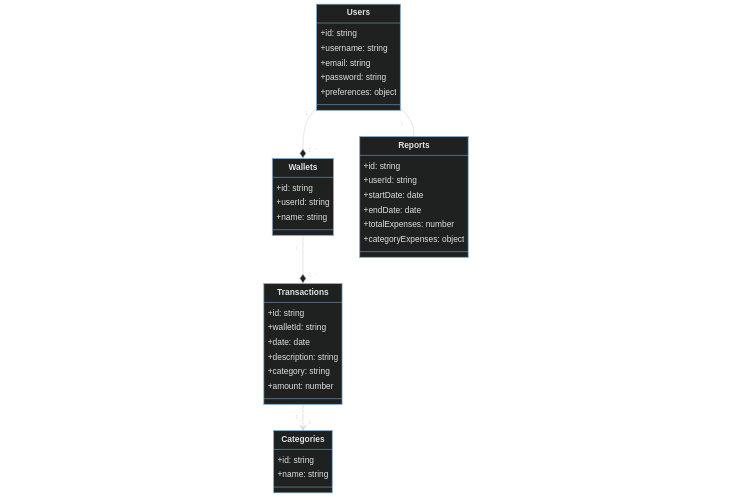
\includegraphics[width=\textwidth]{Diagram/DatabaseUmlDiagram_Reports.png}
    \caption{UML Class Diagram for the Moneager Application}
    \label{fig:class-diagram}
\end{figure}



\section{Strapi Backend Schema Development }
\label{sec:strapi}

In this section, we will explore the backend development of our money management application. We will discuss the various components and provide an overview of the backend architecture.

\subsection{API Endpoints}
We have designed several API endpoints to facilitate data retrieval and manipulation. Here are some examples:

\begin{figure}[htbp]
  \centering
  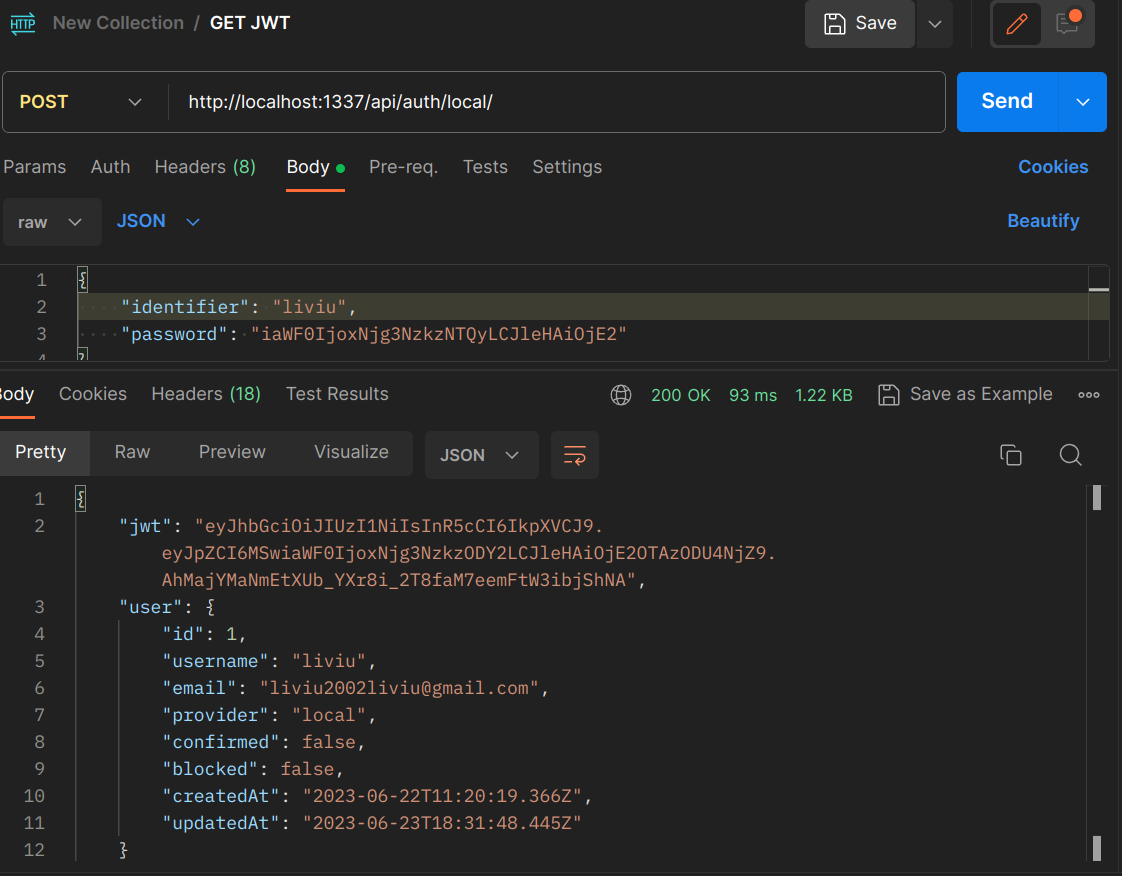
\includegraphics[width=\textwidth]{Strapi/ExampleJWT Get Postman.png}
  \caption{Example of making a JWT authentication request using Postman.}
  \label{fig:example_jwt_postman}
\end{figure}

Figure \ref{fig:example_jwt_postman} demonstrates the process of making a JWT authentication request using Postman. The request is sent to the specified API endpoint, and upon successful authentication, a JSON Web Token (JWT) is returned.

\begin{figure}[htbp]
  \centering
  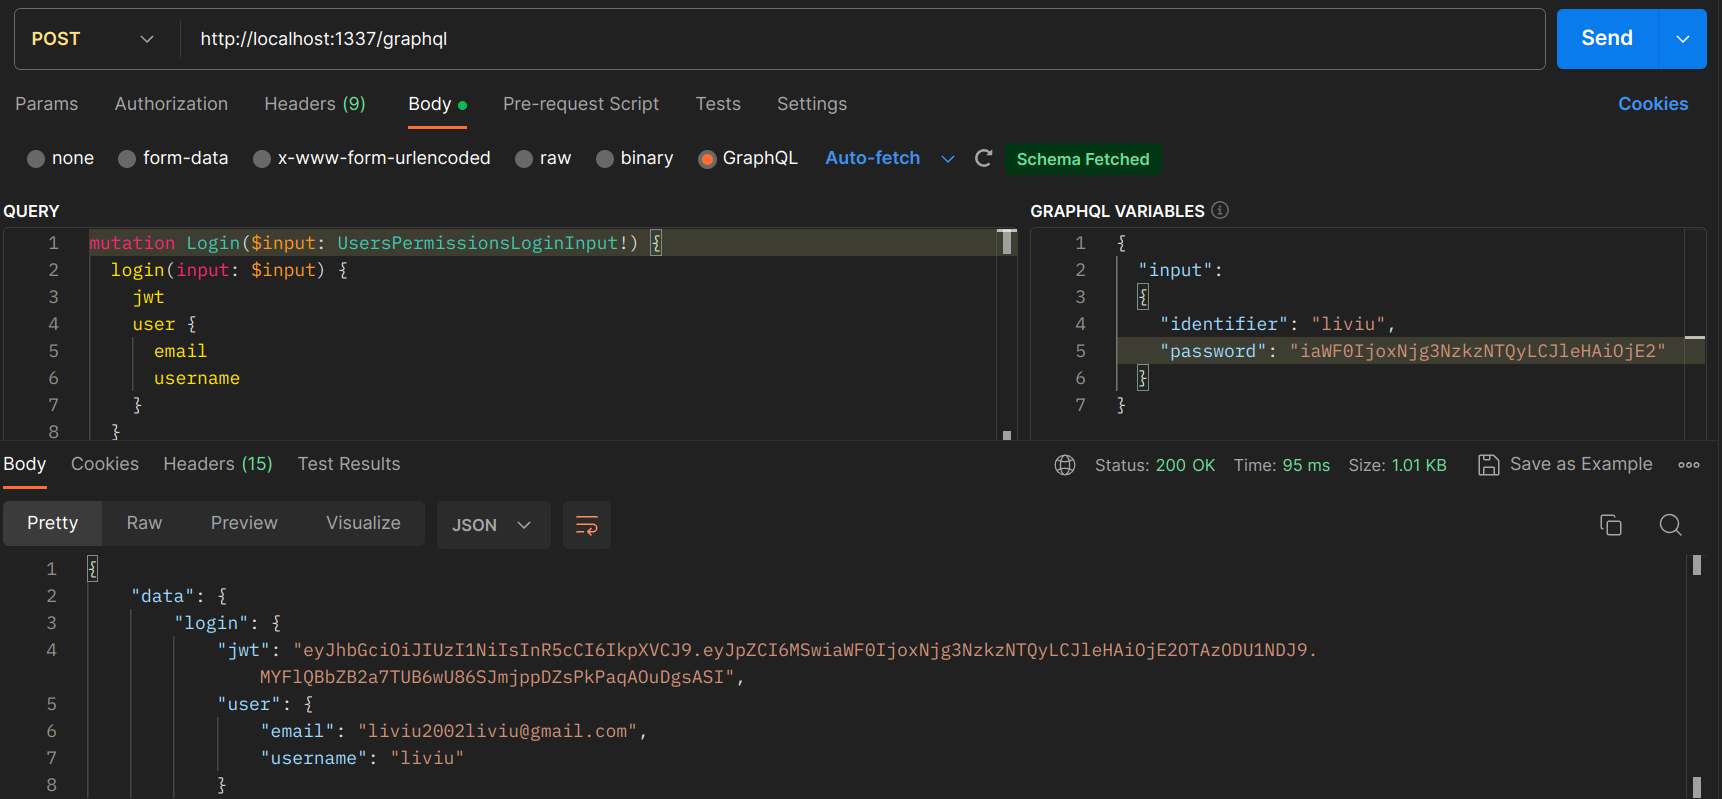
\includegraphics[width=\textwidth]{Strapi/Example of Login using PostMan.png}
  \caption{Example of a login request using Postman.}
  \label{fig:example_login_postman}
\end{figure}

In Figure \ref{fig:example_login_postman}, we showcase an example of a login request using Postman. The user provides their credentials (e.g., email and password), and the backend verifies the information and returns the appropriate response.

\subsection{Database Schema}
Our backend system employs a relational database to store user transactions and related information. The following diagrams illustrate the database schema:

\begin{figure}[htbp]
  \centering
  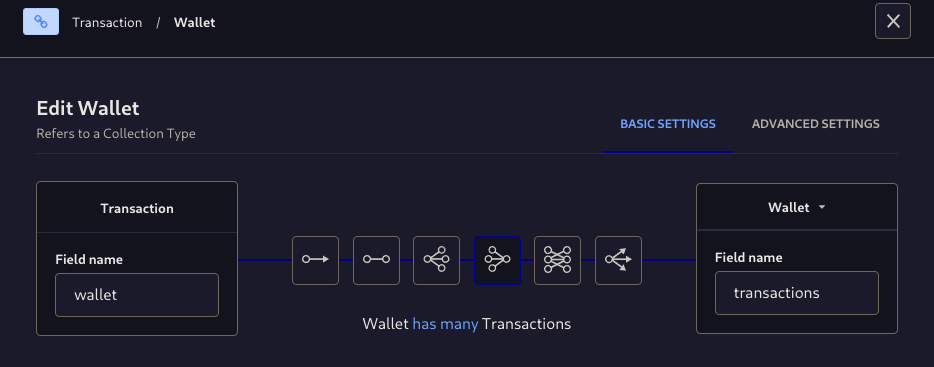
\includegraphics[width=0.8\textwidth]{Strapi/Rel/TransactionToWallet.png}
  \caption{Relationship between transactions and wallets in the database.}
  \label{fig:transaction_wallet_relationship}
\end{figure}

Figure \ref{fig:transaction_wallet_relationship} depicts the relationship between transactions and wallets in the database. Each transaction is associated with a specific wallet, allowing for proper organization and tracking.

\begin{figure}[htbp]
  \centering
  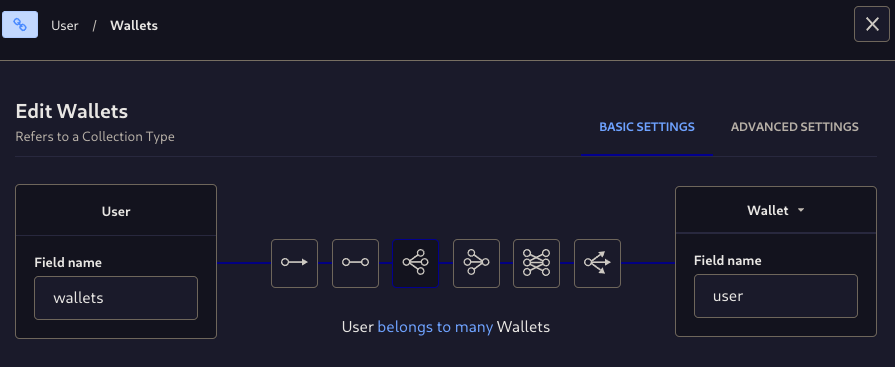
\includegraphics[width=0.8\textwidth]{Strapi/Rel/UserToWallet.png}
  \caption{Relationship between users and wallets in the database.}
  \label{fig:user_wallet_relationship}
\end{figure}

The relationship between users and wallets is illustrated in Figure \ref{fig:user_wallet_relationship}. Each user can have multiple wallets, providing flexibility and customization options.

\subsection{Data Overview}
To provide a better understanding of the backend data, we have included some overview diagrams:

\begin{figure}[htbp]
  \centering
  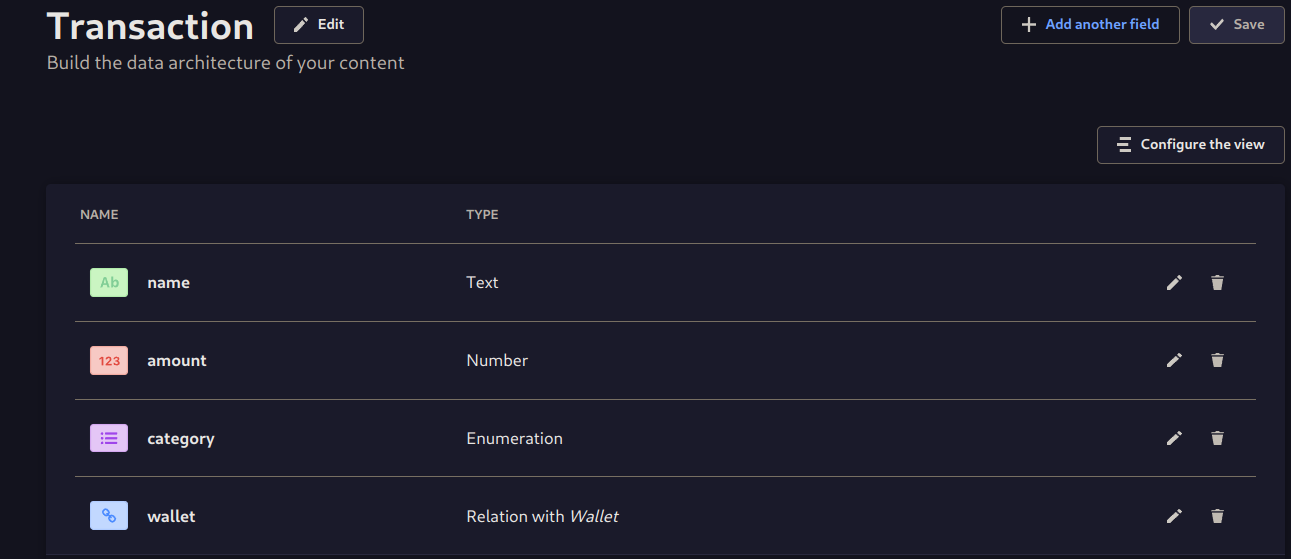
\includegraphics[width=0.6\textwidth]{Strapi/TranOverview.png}
  \caption{Overview of user transactions in the application.}
  \label{fig:transaction_overview}
\end{figure}

Figure \ref{fig:transaction_overview} presents an overview of user transactions within the application. It displays the transaction details and allows for easy tracking and analysis.

\begin{figure}[htbp]
  \centering
  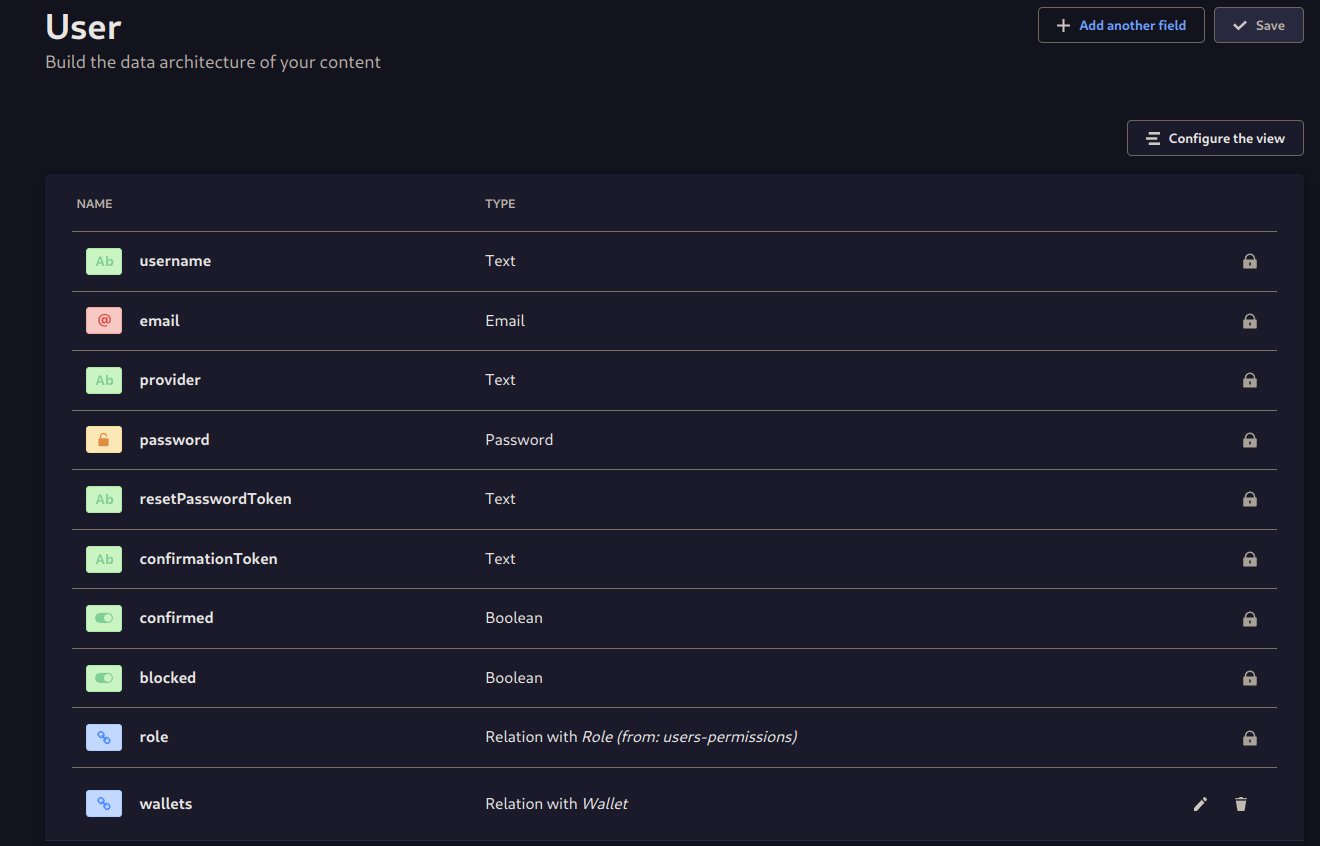
\includegraphics[width=0.6\textwidth]{Strapi/UserOverView.png}
  \caption{Overview of user information in the application.}
  \label{fig:user_overview}
\end{figure}

Lastly, Figure \ref{fig:user_overview} provides an overview of user information stored in the backend. It includes details such as user profiles, authentication data, and associated wallets.

\subsection{Conclusion}
In conclusion, the backend development of our money management application encompasses various API endpoints, a well-defined database schema, and a comprehensive overview of user transactions and data. These components work together to ensure a robust and efficient backend system. By leveraging the power of APIs and a relational database, we enable seamless communication between the frontend and backend, providing users with a seamless and intuitive experience.


\section{GraphQL}
\label{sec:graphql}

GraphQL is a query language for APIs that offers efficient data fetching and flexibility in data querying. We will introduce the concept of GraphQL, discuss its advantages over traditional REST APIs, and demonstrate how to implement GraphQL in our backend.

In this paper, GraphQL was utilized as the query language and runtime for our money management application's backend development. GraphQL played a crucial role in efficiently fetching and manipulating data between the frontend and backend.

By leveraging GraphQL, we were able to establish a clear and structured communication protocol between the client and server. The GraphQL schema defined the available data types, queries, and mutations, serving as a contract between the frontend and backend teams. This schema provided a unified and intuitive way for clients to request specific data and operations.

One of the key benefits of GraphQL was its ability to prevent over-fetching and under-fetching of data. Clients could precisely specify the data they needed in their queries, reducing unnecessary data transfer and improving performance. This granular control over data fetching helped optimize the application's performance and minimize network bandwidth usage.

These are some of the transation used in the aplication:
\newpage
\begin{itemize}
    \item \textbf{CREATE\_WALLET\_MUTATION}:
    \begin{itemize}
        \item Mutation for creating a new wallet.
        \item Input: \texttt{WalletInput} object.
        \item Returns: ID and attributes (amount, name, type) of the created wallet.
        \begin{lstlisting}[language=TypeScript]
        export const CREATE_WALLET_MUTATION = gql`
            mutation CreateWallet($data: WalletInput!) {
                createWallet(data: $data) {
                    data {
                        id
                        attributes {
                            amount
                            name
                            type
                        }
                    }
                }
            }`;
        \end{lstlisting}
    \end{itemize}
    
    \item \textbf{GET\_TRANSACTION\_ENUMS\_QUERY}:
    \begin{itemize}
        \item Query for retrieving transaction category and type enums.
        \item Returns: Enum values for "ENUM\_TRANSACTION\_CATEGORY" and "ENUM\_TRANSACTION\_TYPE".
        \begin{lstlisting}[language=TypeScript]
        export const GET_TRANSACTION_ENUMS_QUERY = gql`
            query GetTransactionEnums {
                categoryEnums: __type(name: "ENUM_TRANSACTION_CATEGORY") {
                    enumValues {
                        name
                    }
                }
                typeEnums: __type(name: "ENUM_TRANSACTION_TYPE") {
                    enumValues {
                        name
                    }
                }
            }`;
        \end{lstlisting}
    \end{itemize}
    
    \item \textbf{CREATE\_TRANSACTION\_MUTATION}:
    \begin{itemize}
        \item Mutation for creating a new transaction.
        \item Input: \texttt{TransactionInput} object.
        \item Returns: ID and attributes (amount, category, name, wallet ID) of the created transaction.
        \begin{lstlisting}[language=TypeScript]
        export const CREATE_TRANSACTION_MUTATION = gql`
            mutation CreateTransaction($data: TransactionInput!) {
                createTransaction(data: $data) {
                    data {
                        attributes {
                            amount
                            category
                            name
                            wallet {
                                data {
                                    id
                                }
                            }
                        }
                        id
                    }
                }
            }`;
        \end{lstlisting}
    \end{itemize}
    
    \item \textbf{UPDATE\_WALLET\_AMOUNT\_MUTATION}:
    \begin{itemize}
        \item Mutation for updating the amount of a specific wallet.
        \item Input: Wallet ID and new amount.
        \item Returns: ID and attributes (amount, name, type) of the updated wallet.
        \begin{lstlisting}[language=TypeScript]
        export const UPDATE_WALLET_AMOUNT_MUTATION = gql`
            mutation UpdateWallet($id: ID!, $amount: Float!) {
                updateWallet(id: $id, data: { amount: $amount }) {
                    data {
                        id
                        attributes {
                            amount
                            name
                            type
                        }
                    }
                }
            }`;
        \end{lstlisting}
            \end{itemize}
    
    \item \textbf{GET\_WALLET\_BALANCE\_QUERY}:
    \begin{itemize}
        \item Query for retrieving the balance of a specific wallet.
        \item Input: Wallet ID.
        \item Returns: Amount of the wallet.
        \begin{lstlisting}[language=TypeScript]
        export const GET_WALLET_BALANCE_QUERY = gql`
            query GetWalletBalanceQUERY($walletId: ID) {
                wallet(id: $walletId) {
                    data {
                        attributes {
                            amount
                        }
                    }
                }
            }`;
        \end{lstlisting}
    \end{itemize}
    
    \item \textbf{GET\_USER\_WALLETS\_QUERY}:
    \begin{itemize}
        \item Query for retrieving wallets associated with a user.
        \item Input: Optional filters (e.g., wallet type).
        \item Returns: IDs, types, and names of user wallets.
    \end{itemize}
    \begin{lstlisting}[language=TypeScript]
    export const GET_USER_WALLETS_QUERY = gql`
        query GetUserWallets($filters: WalletFiltersInput) {
            wallets(filters: $filters) {
                data {
                    id
                    attributes {
                        type
                        name
                    }
                }
            }
        }`;
\end{lstlisting}
    \item \textbf{LOGIN\_MUTATION}:
    \begin{itemize}
        \item Mutation for user login.
        \item Input: \texttt{UsersPermissionsLoginInput} object.
        \item Returns: JWT, user ID, email, and username upon successful login.
        \begin{lstlisting}[language=]
export const LOGIN_MUTATION = gql`
    mutation Login($input: UsersPermissionsLoginInput!) {
        login(input: $input) {
            jwt
            user {
                id
                email
                username
            }
        }
    }`;
\end{lstlisting}
    \end{itemize}
    
    \item \textbf{SIGNUP\_MUTATION}:
    \begin{itemize}
        \item Mutation for user registration.
        \item Input: \texttt{UsersPermissionsRegisterInput} object.
        \item Returns: JWT and user ID upon successful registration.
        \begin{lstlisting}[language=TypeScript]
export const SIGNUP_MUTATION = gql`
    mutation Register($input: UsersPermissionsRegisterInput!) {
        register(input: $input) {
            jwt
            user {
                id
            }
        }
    }`;
\end{lstlisting}
    \end{itemize}


\end{itemize}

\item \textbf{GET\_TRANSACTION\_ENUMS\_QUERY}:
\begin{itemize}
    \item Query for retrieving transaction category and type enums.
    \item Returns: Enum values for "ENUM\_TRANSACTION\_CATEGORY" and "ENUM\_TRANSACTION\_TYPE".
    \begin{lstlisting}[language=TypeScript]
    export const GET_TRANSACTION_ENUMS_QUERY = gql`
        query GetTransactionEnums {
            categoryEnums: __type(name: "ENUM_TRANSACTION_CATEGORY") {
                enumValues {
                    name
                }
            }
            typeEnums: __type(name: "ENUM_TRANSACTION_TYPE") {
                enumValues {
                    name
                }
            }
        }`;
    \end{lstlisting}
\end{itemize}

\item \textbf{CREATE\_TRANSACTION\_MUTATION}:
\begin{itemize}
    \item Mutation for creating a new transaction.
    \item Input: \(\text{{TransactionInput}}\) object.
    \item Returns: ID and attributes (amount, category, name, wallet ID) of the created transaction.
    \begin{lstlisting}[language=TypeScript]
    export const CREATE_TRANSACTION_MUTATION = gql`
        mutation CreateTransaction($data: \text{{TransactionInput}}!) {
            createTransaction(data: $data) {
                data {
                    attributes {
                        amount
                        category
                        name
                        wallet {
                            data {
                                id
                            }
                        }
                    }
                    id
                }
            }
        }`;
    \end{lstlisting}
\end{itemize}

\item \textbf{UPDATE\_WALLET\_AMOUNT\_MUTATION}:
\begin{itemize}
    \item Mutation for updating the amount of a specific wallet.
    \item Input: Wallet ID and new amount.
    \item Returns: ID and attributes (amount, name, type) of the updated wallet.
    \begin{lstlisting}[language=TypeScript]
    export const UPDATE_WALLET_AMOUNT_MUTATION = gql`
        mutation UpdateWallet($id: ID!, $amount: Float!) {
            updateWallet(id: $id, data: { amount: $amount }) {
                data {
                    id
                    attributes {
                        amount
                        name
                        type
                    }
                }
            }
        }`;
    \end{lstlisting}
\end{itemize}

\item \textbf{GET\_WALLET\_BALANCE\_QUERY}:
\begin{itemize}
    \item Query for retrieving the balance of a specific wallet.
    \item Input: Wallet ID.
    \item Returns: Amount of the wallet.
    \begin{lstlisting}[language=TypeScript]
    export const GET_WALLET_BALANCE_QUERY = gql`
        query GetWalletBalanceQUERY($walletId: ID) {
            wallet(id: $walletId) {
                data {
                    attributes {
                        amount
                    }
                }
            }
        }`;
    \end{lstlisting}
\end{itemize}

\item \textbf{GET\_USER\_WALLETS\_QUERY}:
\begin{itemize}
    \item Query for retrieving wallets associated with a user.
    \item Input: Optional filters (e.g., wallet type).
    \item Returns: IDs, types, and names of user wallets.
\end{itemize}
\begin{lstlisting}[language=TypeScript]
export const GET_USER_WALLETS_QUERY = gql`
    query GetUserWallets($filters: WalletFiltersInput) {
        wallets(filters: $filters) {
            data {
                id
                attributes {
                    type
                    name
                }
            }
        }
    }`;
\end{lstlisting}

\item \textbf{GET\_TRANSACTIONS\_QUERY}:
\begin{itemize}
    \item Query for retrieving transactions based on filters.
    \item Input: Transaction filters.
    \item Returns: IDs, attributes (createdAt, amount, category, name, wallet), of the transactions.
    \begin{lstlisting}[language=TypeScript]
    export const GET_TRANSACTIONS_QUERY = gql`
        query GetTransactions($filters: TransactionFiltersInput) {
            transactions(filters: $filters) {
                data {
                    id
                    attributes {
                        createdAt
                        amount
                        category
                        name
                        wallet {
                            data {
                                attributes {
                                    type
                                }
                            }
                        }
                    }
                }
            }
        }`;
    \end{lstlisting}
\end{itemize}

\item \textbf{GET\_WALLET\_BALANCES}:
\begin{itemize}
    \item Query for retrieving the balances of multiple wallets.
    \item Input: Wallet IDs.
    \item Returns: Amounts of the wallets.
    \begin{lstlisting}[language=TypeScript]
    export const GET_WALLET_BALANCES = gql`
        query GetWalletBalanceQUERY($walletId: ID) {
            wallet(id: $walletId) {
                data {
                    attributes {
                        amount
                    }
                }
            }
        }`;
    \end{lstlisting}
\end{itemize}

\item \textbf{GET\_ALL\_WALLETS\_QUERY}:
\begin{itemize}
    \item Query for retrieving all wallets.
    \item Returns: IDs, amounts, and names of all wallets.
    \begin{lstlisting}[language=TypeScript]
    export const GET_ALL_WALLETS_QUERY = gql`
        query GetAllWallets {
            wallets {
                data {
                    id
                    attributes {
                        amount
                        name
                    }
                }
            }
        }`;
    \end{lstlisting}
\end{itemize}

\item \textbf{GET\_ALL\_WALLETS\_QUERY\_NEW}:
\begin{itemize}
    \item Query for retrieving all wallets with additional details (transactions, type).
    \item Input: Optional filters (e.g., wallet type).
    \item Returns: IDs, attributes (amount, name, transactions, type) of all wallets.
    \begin{lstlisting}[language=TypeScript]
    export const GET_ALL_WALLETS_QUERY_NEW = gql`
        query Query_NEW($filters: WalletFiltersInput) {
            wallets(filters: $filters) {
                data {
                    attributes {
                        amount
                        name
                        transactions {
                            data {
                                attributes {
                                    name
                                    updatedAt
                                    amount
                                    category
                                }
                            }
                        }
                        type
                    }
                }
            }
        }`;
    \end{lstlisting}
\end{itemize}

\item \textbf{GET\_ALL\_WALLETS\_QUERY\_sta}:
\begin{itemize}
    \item Query for retrieving all wallets.
    \item Returns: IDs \newpageand amounts of all wallets.
    \begin{lstlisting}[language=TypeScript]
    export const GET_ALL_WALLETS_QUERY_sta = gql`
        query GetAllWallets {
            wallets {
                data {
                    id
                    attributes {
                        amount
                    }
                }
            }
        }`;
    \end{lstlisting}
\end{itemize}

\newpage







